\chapter{Обеспечение надежности ОЭП}
\section{Понятие о надежности приборов и ее обеспечение}

Как было сказано ранее на 1-й лекции, надежность является одним из основных показателей качества ОЭП. Она влияет на рынок изделий, их конкурентоспособность, стоимость, затраты на транспортирование и хранение, обслуживание, безопасность, экологию, расходование природных ресурсов, а также оказывает мощное воздействие на развитие науки и техники в плане создания новых более надежных материалов, элементов и устройств.

Теория надежности приборов, машин, систем и их элементов изложена в многочисленной литературе и обычно преподается студентам в специальных курсах учебных дисциплин. В данном курсе лекций рассматриваются лишь те аспекты надежности, знать которые необходимо конструктору при проектировании ОЭП приборов.

Надежность оптико-электронных приборов достаточно высока, так как они, как правило, содержат небольшое количество подвижных элементов, работают с малыми нагрузками в относительно благоприятных условиях и режимах по сравнению, например, с машинами. Однако обеспечение и повышение их надежности невозможно без проведения специальных мероприятий на этапах проектирования, изготовления и эксплуатации. Рассмотрим основные понятия и показатели надежности изделий.

\textit{Надежность технического изделия} --- его свойство выполнять заданные функции с сохранением эксплуатационных показателей в установленных пределах (т. е. работоспособность), соответствующих заданным режимам и условиям использования, технического обслуживания, хранения и транспортирования в течение требуемого промежутка времени или требуемой наработки.

\textit{Наработка} --- объем или продолжительность работы изделия, которые измеряются в единицах времени, длины, массы, количестве повторных циклов функционирования. Например: наработка выключателей, реле измеряется в числе циклов включения-выключения, наработка двигателей и покрышек автомобиля --- в километрах, наработка источников и приемников излучения, аккумуляторов --- в часах работы.

Надежность изделия обусловливается его безотказностью, ремонтопригодностью, долговечностью и сохраняемостью.

\textit{Безотказность} --- свойство изделия сохранять работоспособное состояние в течение заданного времени или наработки без вынужденных перерывов. Непрерывное сохранение работоспособности в течение заданного времени не исключает некоторых профилактических мероприятий по ее поддержанию (осмотр, чистка, смазка, контроль, тестирование). Безотказность особенно важна для приборов, вынужденный перерыв (отказ) в работе которых связан с опасностью для жизни людей или большими экономическими и экологическими потерями, например для медицинских операционных микроскопов, авиационных приборов, студийных телевизионных камер и космических телескопов, приборов контроля и управления работой атомных электростанций.

Безотказность конкретного прибора измеряется длительностью или объемом выполненной работы до первого отказа. После отказа работоспособность прибора, как правило, может быть восстановлена. Существуют изделия (приборы), принципиально невосстанавливаемые после отказа, например приборы спутников связи, ряд унифицированных электронных блоков и другие изделия однократного использования. Обнаружение причин отказа и последующее восстановление зависят от конструкции прибора, характера отказа и связаны с показателями ремонтопригодности.

\textit{Ремонтопригодность} --- свойство изделия, заключающееся в его приспособленности к предупреждению, обнаружению и устранению отказов, а также поддержанию работоспособности путем технического обслуживания и ремонтов. Ремонтопригодность характеризуется затратами времени и средств на восстановление изделия после отказа и поддержание его в работоспособном состоянии.

Ремонтопригодность прибора закладывается на этапе разработки его конструкции (особенно при компоновке), обеспечивающей доступность к малонадежным элементам, контролепригодность, легкозаменяемость, удобство и простоту (рациональность) обслуживания и ремонта.

\textit{Долговечность} --- свойство изделия сохранять работоспособность до наступления предельного состояния, т.е. способность к длительной эксплуатации при проведении необходимого технического обслуживания и ремонтов.

Предельное состояние --- состояние, при котором дальнейшее использование изделия по назначению невозможно, недопустимо или нецелесообразно. Данное состояние наступает в случаях: когда после отказа прибора его невозможно восстановить либо невозможно достичь требуемых показателей качества (например, точности); когда безопасность эксплуатации прибора ухудшается до недопустимых пределов; когда восстановление изделия после отказа экономически нецелесообразно либо его дальнейшая эксплуатация экономически не эффективна, так как он морально устарел и не обеспечивает необходимых производительности работы, сервиса, энергоемкости, габаритных размеров.

Хорошей иллюстрацией сокращения долговечности приборов из-за их морального устаревания являются такие бытовые приборы, как телевизоры, любительские видеокамеры, мобильные телефоны, персональные компьютеры (замена которых чаще всего происходит при появлении новых, более совершенных моделей, а не по причине их отказа).

Долговечность изделий характеризуется техническим ресурсом --- наработкой до предельного состояния.

Заметим, что для невосстанавливаемых объектов значения понятий долговечности и безотказности совпадают.

\textit{Сохраняемость} --- свойство изделия сохранять значения показателей безотказности, ремонтопригодности и долговечности (т.е. эксплуатационные показатели) в течение и после хранения и транспортирования.

Подавляющее большинство приборов поступает к потребителю, пройдя стадии хранения (на фирме-изготовителе, на складах, в магазинах) и транспортировки (автомобильным, железнодорожным, воздушным и водным транспортом), во время которых прибор подвергается различным воздействиям: механическим нагрузкам (статическим и динамическим), климатическим (осадки, температура, давление, влажность и запыленность воздуха), биологическим (микроорганизмы, насекомые, грызуны), радиационным и химическим. В результате эксплуатационные показатели и характеристики приборов могут ухудшиться или же изменится вероятность их появления.

Наиболее эффективные методы повышения сохраняемости связаны с правильной конструкцией упаковки, консервацией, применением специальных защитных покрытий, профилактическим обслуживанием при хранении, а также с повышением культуры работы транспортных и складских служб.
Одним из важнейших понятий надежности является понятие отказа.

\textit{Отказом} называют неисправность, без устранения которой невозможно дальнейшее выполнение изделием всех или хотя бы одной из его основных функций, т.е. нарушение работоспособного состояния изделия 

Если возникла неисправность, не связанная с эксплуатационными показателями, например царапины и небольшие вмятины на корпусе прибора, отслоение краски, поломка фиксатора переносной рукоятки, перегорание сигнальной лампочки, утеря запасного элемента, коррозия неответственной детали, то это событие называют повреждением или дефектом, приводящим прибор в неисправное состояние (но работоспособное), так как он не будет соответствовать всем требованиям технической документации.

Отказы классифицируются по ряду признаков на следующие виды (рис.~\ref{pic:13otkaz}).

\begin{figure}[h!]
	\caption{ Виды отказов }
	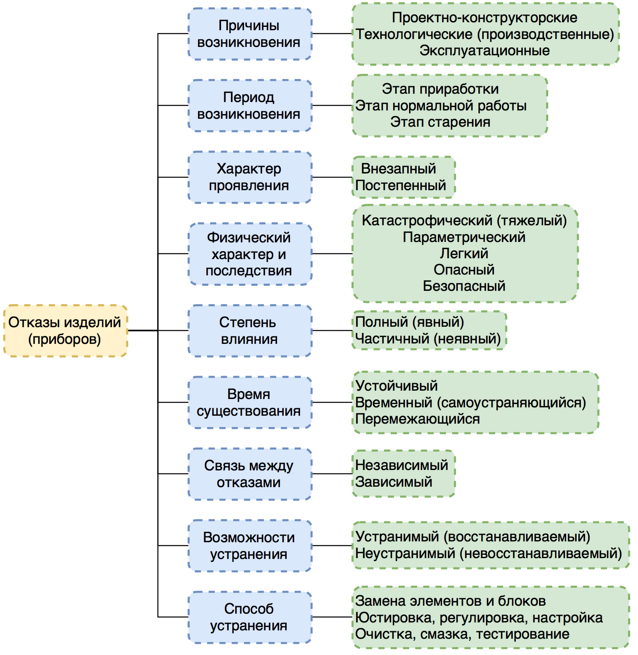
\includegraphics[width=0.7\textwidth]{13otkaz.png}
	\label{pic:13otkaz}
\end{figure}

По причинам возникновения: 
\begin{itemize}
\item Проектно-конструкторскими причинами отказов являются ошибки, заложенные в концепцию, структуру или конструкцию элементов прибора [например: физический принцип работы и структура прибора не согласованы с условиями его эксплуатации (наличие электромагнитных полей, динамических нагрузок, климатических воздействий); неправильно выполнена компоновка (источник излучения нагревает эталонные элементы); неудачно выбран материал деталей и неправильно рассчитаны допуски на погрешности их размеров (деформации или децентрировки оптических деталей в оправах при колебаниях температуры)].
\item Технологическими или производственными причинами отказов являются нарушения технологических процессов изготовления и сборки деталей, дефекты материалов и комплектующих, а также отступления от инструкций и методик юстировки, калибровки, аттестации и испытаний приборов (например, расклейка деталей из-за того, что они не были обезжирены перед склейкой, или вследствие применения клея с истекшим сроком использования).
\item Эксплуатационными причинами отказов являются ошибки операторов, эксплуатация приборов при недопустимых условиях и режимах, износ и старение элементов.
\end{itemize}

По периоду возникновения:
\begin{itemize}
\item Отказы этапа приработки --- отказы, возникающие в начальный период эксплуатации изделия и обусловленные, как правило, проектно-производственными ошибками и погрешностями; поэтому их называют часто конструкторско-технологическими отказами.
\item Отказы этапа нормальной работы --- отказы, появляющиеся после периода приработки (рис.~\ref{pic:13freqotkaz}~б).
\item Отказы этапа старения --- отказы, обусловленные старением, износом и коррозией элементов.
\end{itemize}

По характеру проявления:
\begin{itemize}
\item Внезапный отказ --- отказ, который появляется внезапно в результате резкого, скачкообразного изменения основных параметров прибора под воздействием факторов, связанных с внутренними дефектами его элементов или с ошибками оператора, и который предвидеть и предупредить очень трудно; чаще всего внезапные отказы происходят в начальный период эксплуатации прибора [$ f(t) $ -- дифференциальная (плотность вероятности) функция распределения случайного времени работы прибора до наступления внезапного отказа на этом этапе обычно носит экспоненциальный характер (рис.~\ref{pic:13lawotkaz}~а)].
\item Постепенный отказ --- отказ, при котором наблюдается постепенное изменение параметров прибора в результате естественного старения, износа, коррозии, запыленности его элементов [например: отказ по точности вследствие износа направляющих подвижных функциональных систем прибора; заклинивание (или увеличение моментов вращения) окуляров бинокля из-за загустевания смазочного материала; ухудшение контраста изображения из-за старения трубки видикона телекамеры или трубки монитора); так как параметры элементов прибора ухудшаются постепенно, то данный отказ можно предвидеть и предупредить (например, профилактической заменой элементов, срок эксплуатации которых приближается к предельному)]; естественно, что постепенный отказ не может произойти при испытаниях прибора или на этапе приработки [закон распределения случайного времени работы прибора до появления постепенного отказа обычно близок к нормальному (рис.~\ref{pic:13lawotkaz}~б)].
\end{itemize}
 
\begin{figure}[h!]
	\caption{ Законы распределения отказов }
	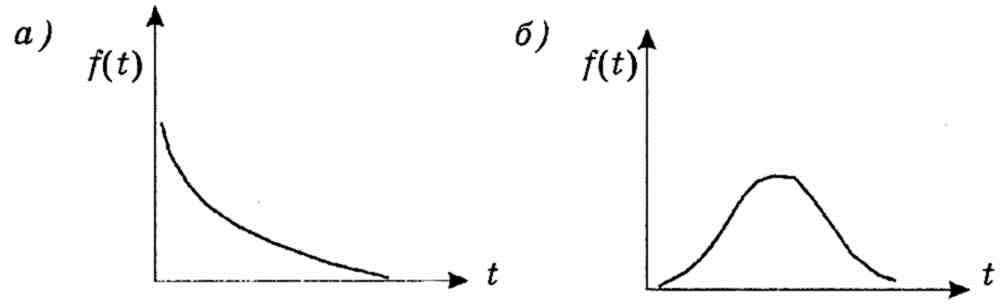
\includegraphics[width=1\textwidth]{13lawotkaz.png}
	\label{pic:13lawotkaz}
\end{figure}

По степени влияния и последствиям:
\begin{itemize}
\item Полный отказ (явный) --- отказ, при возникновении которого невозможно использовать прибор по прямому назначению до устранения причины отказа (например: перегорела лампочка подсветки марки автоколлиматора);
\item частичный отказ (неявный) --- отказ, связанный с ухудшением какой-либо одной из характеристик прибора, при котором возможно частичное использование изделия по прямому назначению (например: невозможность включения светофильтра для повышения контраста изображения; появление осыпки в поле зрения; возникновение bad-секторов на дисках компьютера).
\end{itemize}

По физическому характеру и последствиям:
\begin{itemize}
\item Катастрофический отказ (тяжелый) --- отказ прибора, приводящий к полному нарушению его работоспособности, устранение которого связано с большими экономическими и временными затратами [например: разрушение оптических элементов; полная разъюстировка систем; поломки; деформации, заклинивания подвижных частей прибора (винчестера в компьютере); короткое замыкание в электросхемах (системной плате)].
\item Параметрический отказ --- отказ, при котором прибор выполняет все свои основные функции, но один из эксплуатационных параметров (показателей) вышел за границу допустимых значений [например: увеличился шум работы прибора, появился разворот (расфокусировка) изображения, ухудшилась точность функционирования]; часто параметрический отказ (особенно по точности) удается обнаружить не сразу, что может привести к нежелательным последствиям (например, к выпуску бракованной продукции).
\item Легкий отказ - отказ, устранение которого не связано со значительными экономическими и временными затратами и не требует привлечения ремонтных служб (например: замена предохранителей, источников излучения, элементов питания, тестирование программ после сбоя).
\item Опасный отказ --- отказ, который связан с опасностью для жизни или здоровья людей, а также с экологическими катастрофами.
\item Безопасный отказ --- отказ, который не связан с опасностью для жизни или здоровья людей, а также с экологическими катастрофами.
\end{itemize}

По связи между отказами:
\begin{itemize}
\item независимый отказ --- отказ, который не является причиной других отказов;
\item зависимый отказ --- отказ, который возникает из-за других отказов [например: уменьшение срока службы лампы подсветки при подаче на нее напряжения выше номинального из-за сбоя регулировки блока питания; заклинивание гайки винтового механизма при поломке ограничителя вращения винта (двигателя)].
\end{itemize}

По времени существования:
\begin{itemize}
\item устойчивый отказ - отказ, который устраняется только в результате ремонта, регулировки (тестирования) или замены отказавших элементов и блоков прибора;
\item временный (самоустраняющийся) отказ --- отказ, самопроизвольно устраняющийся, без вмешательства обслуживающего персонала, вследствие исчезновения вызвавшей его причины; возникает часто из-за нарушения режимов или условий работы (например: из-за запотевания оптических деталей; из-за расфокусировки, обусловленной перепадом температуры; потеря точности из-за недопустимых внешних вибраций прибора);
\item перемежающиеся отказы (сбои) --- внезапно повторяющиеся непродолжительные самоустраняющиеся отказы, которые свидетельствуют о наличии ненормальности в элементах прибора, программах или режимах и условиях его работы (например: нарушение контакта лампочки подсветки, обусловленное ослаблением крепления и вибрациями прибора; погрешность некоторых результатов измерений из-за вируса в памяти приборного компьютера). 
\end{itemize}

По возможности устранения: 
\begin{itemize}
\item устранимый отказ --- отказ, который подлежит устранению и может быть устранен;
\item неустранимый отказ --- отказ, не подлежащий устранению (невосстанавливаемые объекты) или не поддающийся устранению.
\end{itemize}

По способу устранения:
\begin{itemize}
\item заменой элементов и блоков (из входящих в комплект прибора или приобретаемых);
\item юстировкой, регулировкой или настройкой отказавшего элемента или всего прибора;
\item организационно-техническими мероприятиями: очисткой, смазкой, тестированием (<<лечением>>).
\end{itemize}

%\section{Основные единичные показатели надежности \\приборов}

Единичные показатели надежности являются количественными характеристиками безотказности, ремонтопригодности, долговечности или сохраняемости приборов в определенных условиях. Рассмотрим некоторые из этих показателей.

\begin{flushleft}
\textbf{Показатели безотказности}
\end{flushleft}

Эти показатели являются количественными характеристиками законов распределения случайного времени безотказной работы прибора или случайного числа отказов за определенное время или наработки.

Наиболее общей характеристикой случайного времени работы (наработки) прибора до появления отказа является вероятность безотказной работы $ P(t) $~--- вероятность того, что в заданный интервал времени (заданное число циклов повторного функционирования) и при заданных режимах и условиях эксплуатации не произойдет отказа:
\[ P(t) = 1 - F(t) = 1 - \int\limits_{-\infty}^{t}f(t)\,dt = \int\limits_{t}^{\infty}f(t)\,dt, \]
где $ F(t) $ и $ f(t) $ --- интегральная и дифференциальная (плотность вероятности) функции распределения случайного времени работы (наработки) прибора до первого отказа.

Если функция распределения случайного значения времени $ t $ до первого отказа подчиняется экспоненциальному закону $ F(t) = 1 - e^{-\lambda\,t} $ (этап приработки), то вероятность определится следующим выражением:
\[ P(t) = 1 - (1-e^{-\lambda\,t})\int\limits_{t}^{\infty}\lambda\,e^{-\lambda\,t}\,dt = e^{-\lambda\,t} = e^{-\dfrac{t}{t_\text{ср}}}, \]
где $ \lambda = \dfrac{1}{t_\text{ср}} $ -- параметр распределения; $ t_\text{ср} $ -- среднее значение времени (средняя наработка) работы прибора до отказа; $ f(t) = \lambda e^{-\lambda\,t} $ -- плотность вероятности экспоненциального распределения.

Для нормального закона распределения F(t) (этап старения) вероятность будет
\[ P(t) = 1 - \dfrac{1}{\sigma_t\sqrt{2\pi}}\int\limits_{-\infty}^{t}e^{\dfrac{-(t-t_\text{ср})^2}{2\sigma_t^2}}\,dt, \]
где $ \sigma_t $ -- среднее квадратическое отклонение случайного времени (наработки) прибора до первого отказа.

Статистическая вероятность безотказной работы может быть вычислена по формуле:
\[ P(t) = \lim\limits_{\substack{\Delta t \rightarrow 0 \\ N_0 \rightarrow\infty}} \dfrac{N_0 - \sum\limits_{i=1}^{m}n_i}{N_0} = 
1 - \sum\limits_{i=1}^{m} \dfrac{n_i}{N_0} = 1 -F(t), \]
где $ N_0 $ -- число приборов в начале эксплуатации (испытания); $ n_i $ -- число приборов, отказавших в i-м интервале времени; $ m = t/\Delta t $~-- число интервалов; $ t $ -- время эксплуатации; $ \Delta t $ -- продолжительность интервала времени; $ F(t) = \sum\limits_{i=1}^{m}\dfrac{n_i}{N_0} $~-- статистическая вероятность отказа прибора.

Чем больше $ N_0 $ и меньше $ \Delta t $, тем ближе статистическая вероятность безотказной работы к теоретической.

На рис.~\ref{pic:13probabilityotkaz} показаны типичные изменения вероятности безотказной работы~1 и вероятности отказа~2 прибора во времени.

\begin{figure}[h!]
	\caption{ Графики изменения вероятности отказа и безотказной работы }
	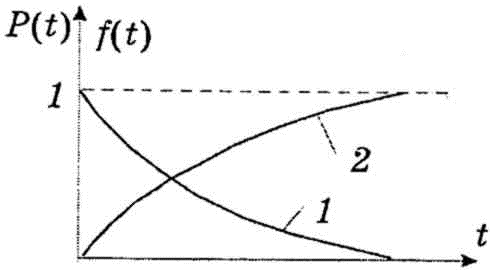
\includegraphics[width=0.6\textwidth]{13probabilityotkaz.png}
	\label{pic:13probabilityotkaz}
\end{figure}

Другим нормируемым показателем безотказности является среднее время безотказной работы $ t_\text{ср} $ (средняя наработка до отказа) --- ожидаемое время исправной работы прибора до появления первого отказа:
\[ t_\text{ср} = \int\limits_{0}^{\infty} t \, f(t)\, dt = \int\limits_{0}^{\infty} P(t)dt \approx \dfrac{\sum\limits_{i}^{m}n_i\,t_\text{cр i}}{N_0} = \sum\limits_{j}^{N_0} \dfrac{t_j}{N_0}, \]
где $ t_\text{cр i} = \dfrac{t_i - t_{i-1}}{2};\,t_{i-1},\,t_i $ --- значения времени в начале и в конце i-ro интервала; $ t_j $ --- время работы (наработки) до первого отказа j-го прибора.

Важными характеристиками безотказности являются \textit{частота и интенсивность отказов}.

\textit{Частотой отказов} (плотностью распределения времени работы прибора до отказа) по статистической информации называют отношение числа приборов, отказавших в единицу времени $ n\,\Delta t/\Delta t $ к числу приборов в начале эксплуатации (испытания) $ N_0 $ при условии, что отказавшие приборы не восстанавливаются и не заменяются:
\[ f(t)\approx \dfrac{n(t+\Delta t) - n(t)}{N_0 \, \Delta t} = \dfrac{n(\Delta t)}{N_0 \Delta t},   \]
где $ n(t) $ -- число приборов, отказавших за время $ t $, $ n(\Delta t) $ -- число приборов, отказавших в интервал времени $ \Delta t $.
На рис.~\ref{pic:13freqotkaz}~а представлен статистический график (гистограмма) частоты отказов.

\begin{figure}[h!]
	\caption{ Графики частоты (а) и интенсивности (б) отказов }
	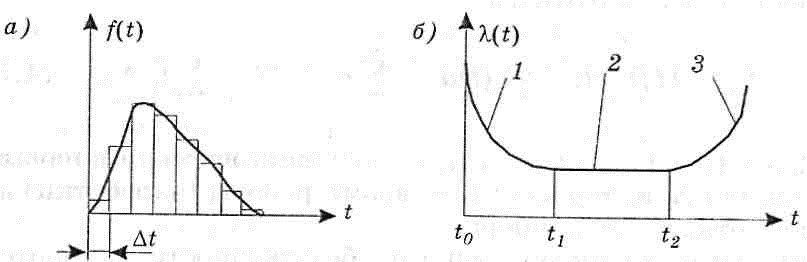
\includegraphics[width=1\textwidth]{13freqotkaz.png}
	\label{pic:13freqotkaz}
\end{figure}

\textit{Интенсивностью отказов $ \lambda(t) $} называют отношение числа приборов, отказавших в единицу времени, к числу приборов, работоспособных в данный момент (интервал) времени $ N_t $:
\[ \lambda (t) \approx \dfrac{n(t+\Delta t) - n(t)}{N_t\Delta t} = \dfrac{n(\Delta t)}{N_t\Delta t}. \]

Эта характеристика показывает, какая часть приборов по отношению к среднему числу исправно работающих выходит из строя из-за отказов в единицу времени (обычно в час).

Типичная кривая изменения интенсивности отказов в единицу времени, характерная для случая внезапных отказов, приведена на рис.~\ref{pic:13freqotkaz}~б. Здесь выделены три периода интенсивности отказов: начальный период от $ t_0 $ до $ t_1 $ (этап приработки~-- 1), второй период времени от $ t_1 $ до $ t_2 $ (этап нормальной работы~-- 2) и третий период после времени $ t_2 $ (этап старения~-- 3).

В начальном периоде интенсивность отказов приборов выше, чем в нормальный период работы, что объясняется проектно-производственными ошибками и погрешностями, дефектами материалов и покупных (унифицированных) изделий. Продолжительность этого периода конструкторско-технологических отказов зависит от типа прибора, его сложности, количества унифицированных элементов и узлов, условий производства, условий эксплуатации.

Период нормальной работы характеризуется более высокой и стабильной надежностью. Интенсивность отказов здесь постоянна и обусловлена эксплуатационными факторами: ошибками операторов, скачками напряжений в электрической сети, ухудшением условий и режимов эксплуатации (перегрузки, воздействие внешней среды). Продолжительность этого этапа различна для приборов, основанных на разных физических принципах (электронных, оптико-механических, механических, электронно-механических, оптико-электронных) и работающих в разных режимах и условиях. Например, продолжительность этапа нормальной работы механических приборов и узлов существенно меньше подобного этапа работы электронных приборов.

Период старения характеризуется резким возрастанием интенсивности отказов, что вызвано износом отдельных деталей, их коррозией, загрязнением, старением материалов, расходованием ресурса элементов. Продолжительность данного этапа также зависит от вида приборов, их конструкции, качества используемых материалов, условий и режимов эксплуатации, а также технического обслуживания и профилактических мероприятий.

На рис.~\ref{pic:13robust} и рис.~\ref{pic:13quality} приведены графики характеристик безотказности для экспоненциального и нормального соответственно законов распределения случайного времени (наработки) работы прибора между отказами. Заметим, что интенсивность отказов при экспоненциальном распределении является постоянной величиной, а при нормальном распределении~--- монотонно возрастает в функции времени (наработки).

\begin{figure}[h!]
	\caption{ Графики характеристик надежности --- экспоненциальный закон распределения времени наработки прибора }
	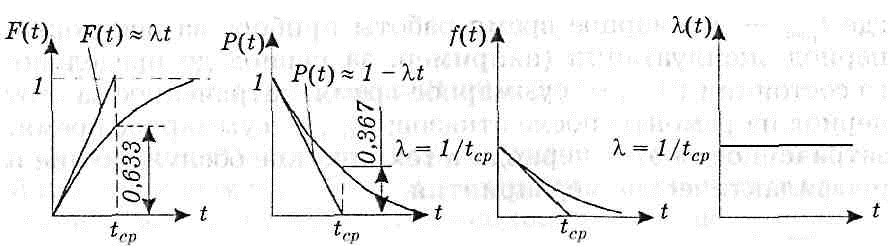
\includegraphics[width=1\textwidth]{13robust.png}
	\label{pic:13robust}
\end{figure}

\begin{figure}[h!]
	\caption{ Графики характеристик надежности - нормальный .закон распределения времени наработки прибора }
	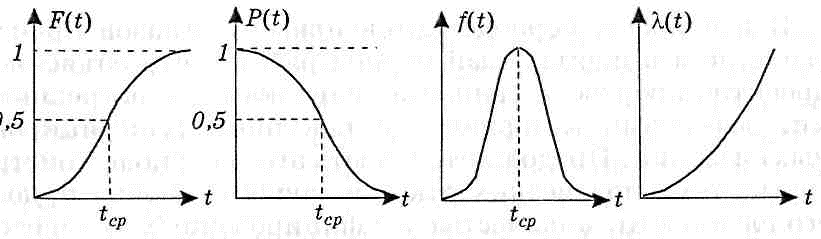
\includegraphics[width=1\textwidth]{13quality.png}
	\label{pic:13quality}
\end{figure}

\begin{flushleft}
\textbf{Показатели ремонтопригодности}
\end{flushleft}

Эти показатели характеризуют затраты времени и средств на техническое обслуживание и ремонт прибора. В качестве таковых используют, например, \textit{коэффициенты готовности и технического использования}. Эти показатели используются не только как единичные, но и как комплексные показатели надежности.

\textit{Коэффициент готовности} характеризует потери времени на восстановление прибора и равен вероятности того, что прибор работоспособен в любой момент времени в промежутках между плановым обслуживанием:
\[ K_\text{г} = \dfrac{t_\text{ср}}{T_\text{в} + t_\text{ср}}, \]
где $ T_\text{в} $~-- среднее время восстановления, $ t_\text{ср} $~-- средняя наработка прибора на отказ.

\textit{Коэффициент технического использования} более полно отражает потери времени из-за ненадежности прибора:
\[ K_\text{т} = \dfrac{t_\text{раб}}{t_\text{раб} + t_\text{рем} + t_\text{обсл}}, \]
где $ t_\text{раб} $~-- суммарное время работы прибора за некоторый период эксплуатации (например, за период до предельного состояния), $ t_\text{рем} $~-- суммарное время, затраченное за этот период на ремонты после отказов; $ t_\text{обсл} $~-- суммарное время, затраченное за этот период на техническое обслуживание и профилактические мероприятия.

Кроме потерь времени ненадежность прибора приводит к материальным затратам на ремонт и поддержание прибора в работоспособном состоянии. Поэтому существуют также экономические показатели ремонтопригодности, характеризующие стоимость ремонтов и технического обслуживания прибора за определенный период эксплуатации.

\begin{flushleft}
\textbf{Показатели сохраняемости}
\end{flushleft}

Показатели сохраняемости дают количественную характеристику способности прибора сохранять безотказность и другие показатели качества при хранении и транспортировке в определенных условиях. Такими показателями являются, например, \textit{коэффициент сохранения безотказности} и \textit{коэффициент сохраняемости}.

\textit{Коэффициент сохранения безотказности} определяется отношением вероятности безотказной работы нового прибора в течение некоторого времени (или наработки) $ t_0 $ после хранения и транспортировки $ P_1(t_0) $ к этой же вероятности до хранения и транспортировки $ P_0(t_0) $:
\[ L_c = \dfrac{P_1(t_0)}{P_0(t_0)}. \]

Коэффициент сохраняемости определяется по следующей формуле:
\[ K_c =  \prod\limits_{i=1}^{n} \dfrac{Q'_i - Q_{i \text{доп}}}{Q^0_i - Q_{i \text{доп}}},   \]
где $ Q^0_i $ и $ Q'_i $~-- значения независимых показателей качества прибора (например, точности, дальности действия, мощности) до и после его хранения и транспортирования, $ Q_{i \text{доп}} $~-- предельно допустимое значение этих показателей.

\newpage
\begin{flushleft}
\textbf{Показатели долговечности}
\end{flushleft}

Долговечность прибора характеризуется его ресурсом~--- общим временем или объемом работы за весь срок службы до момента, когда потребуются его списание из-за невозможности дальнейшей эксплуатации (предельное состояние) или капитальный ремонт.

Для определения рассмотренных выше показателей надежности необходимо знать распределение случайного времени между отказами, которое подчиняется обычно законам распределения Гаусса, экспоненциальному, Релея, гамма-распределению, Вейбулла и их суперпозиции. Эти законы распределения используются при вычислении тех или иных показателей надежности в зависимости от типа приборов (электронные, электромеханические, оптико-механические, оптико-электронные), периода эксплуатации прибора (этапы приработки, нормальной работы, старения), вида отказов (внезапный, постепенный, катастрофический, зависимый), условий эксплуатации.

\section{Обеспечение надежности приборов}

Надежность прибора закладывается на этапах проектно-конструкторской работы и обеспечивается в процессе его изготовления и эксплуатации. Рассмотрим некоторые факторы, которые нужно учитывать, и мероприятия, которые нужно выполнять для обеспечения и повышения показателей надежности приборов.

\begin{flushleft}
\textbf{Проектно-конструкторские мероприятия для повышения надежности}
\end{flushleft}

\begin{enumerate}
\item При поиске идей и разработке принципа функционирования прибора необходимо учитывать надежность тех физических эффектов, которые будут заложены в основу его работы. Например, приборы для измерения длин, основанные на интерференции света (интерферометры) и работающие в цеховых условиях, будут менее надежны (из-за чувствительности к колебанию температуры, давлению и влажности воздуха, вибрациям) по сравнению с ОЭП, основанными на фотоэлектрических и телевизионных преобразователях (датчиках) линейных перемещений и расстояний, которые менее чувствительны к влияющим факторам.
\item При разработке структуры и конструкции прибора следует использовать как можно больше известных (заимствованных) конструктивных решений, унифицированных и стандартизированных функциональных устройств, узлов и элементов.
Использование заимствованных решений и унифицированных устройств повышает надежность прибора, так как они проверены практикой и лучше отработаны в схемном, конструктивном и технологическом отношениях.
\item Для ответственных элементов прибора необходимо использовать высококачественные материалы и комплектующие изделия, которые обязательно должны выбираться с учетом условий и режимов его работы. Например, неправильный выбор материалов прибора, работающего в тропиках, существенно уменьшает срок его службы (ресурс) и может привести к катастрофическому отказу. Применение пластмасс для ответственных деталей (линз, кулачков, зубчатых колес) или интенсивно работающих вспомогательных элементов (переключателей, фиксаторов), как правило, снижает надежность прибора, так как многие виды полимеров подвержены старению во времени (т.е. изменению структуры и химического состава, сопровождающемуся изменением механических, физических и химических свойств) под воздействием внешних факторов --- солнечного света, температуры, кислорода, озона, влаги, ионизирующих излучений, проникающей радиации, механических напряжений, биологических и химических воздействий среды.

Ответственные детали приборов должны подвергаться необходимой термической обработке (закалка, отжиг, старение), покрытиям, смазке, консервирующей защите, что существенно повышает показатели надежности всего прибора. Сочетания материалов деталей в соединениях не должны образовывать гальванические пары.
\item Разрабатывая конструкцию прибора, необходимо соблюдать принципы конструирования, оказывающие влияние на его функциональную и точностную надежность (например, принцип отсутствия избыточного базирования в соединениях деталей, принцип учета тепловых свойств соединяемых деталей, принцип кратчайшей цепи преобразования, принцип отсутствия избыточных связей в механизмах и приводах).
При определении размеров и посадок деталей следует учитывать условия жесткости, износоустойчивости, отсутствие заклинивания, деформаций.
\item В конструкции прибора необходимо предусмотреть разнообразные защитные устройства, которые можно подразделить на следующие группы:
\begin{itemize}
\item устройства, предохраняющие прибор от аварийного состояния при отказе того или иного элемента прибора, ошибках оператора, колебании электрического напряжения в сети (например: автоматические выключатели и плавкие предохранители в цепи питания; защитные колпачки и блокираторы случайного нажатия кнопок включения (выключения) прибора, перехода на решение тестовых программ ЭВМ; компьютерные программы защиты от несанкционированного доступа в систему управления прибором или ошибок при вводе значений параметров);
\item устройства, предотвращающие подключение низковольтных источников света, фотоприемников и другого электрооборудования прибора в бытовую сеть либо к несоответствующим гнездам электронных блоков [например, типичными и частыми ошибками являются использование стандартной вилки для подключения источника излучения (лампы подсветки напряжением 6-8 Вт) к блоку питания, которую по ошибке можно включить в бытовую сеть, а также несоблюдение полярности питающего напряжения некоторых приемников излучения, приводящее к выходу прибора из строя или снижению порога его чувствительности];
\item устройства, предотвращающие съем «несъемных» наружных элементов без специального инструмента и приспособлений (окуляров, объективов, рукояток управления), а также потерю «съемных» элементов и их крепежа (невыпадающие винты, поддерживающие цепочки, магнитные фиксаторы крышек, кожухов, бленд, светофильтров);
\item устройства, предохраняющие наружные оптические детали от механического повреждения и загрязнения, а также исключающие возможность воздействия на органы управления и регулирования посторонними предметами (защитные кожухи, диафрагмы, экраны);
\item устройства, предотвращающие порчу прибора при хранении и транспортировке от влияния влаги, грызунов, плесени и грибков, тряски и вибрации (устройства вентиляции, принудительного продува, осушки, амортизации, защитные металлические сетки).
\end{itemize}
\item Конструкция прибора должна обеспечивать доступность всех его компонентов, узлов и деталей для осмотра, контроля, обслуживания, регулировки или замены. Замена или регулировка малонадежных элементов прибора не должна приводить к разборке других узлов. Например, замена перегоревшего источника освещения не должна быть связана со съемом конденсора или разборкой части прибора для доступа к нему.
\item В приборе должны быть предусмотрены световые и звуковые индикаторы включения питания и технического состояния прибора, сигнализирующие о разряде источников энергии, перегрузке, отказе двигателей, перегреве или переохлаждении, выходе из нормального режима эксплуатации, сбое программы вычислений, превышении допустимой погрешности измерений.
\item Весьма эффективным приемом повышения надежности приборов является резервирование, под которым понимается использование дополнительных (дублирующих) элементов, средств и возможностей в целях сохранения работоспособного состояния прибора при отказе одного или нескольких его элементов.

Дублирование малонадежных элементов или устройств в технических изделиях применяется достаточно давно и подсказано самой природой, которая заложила дублирование, например, важных органов и чувств человека и животных.

Кратностью резервирования называют отношение числа резервных элементов (изделий) к числу основных.

Различают резервирование следующих видов:
\begin{itemize}
\item общее -- резервирование прибора (изделия) в целом;
\item раздельное -- поэлементное;
\item постоянное -- без перестройки структуры прибора в случае отказа его элементов;
\item динамическое -- с перестройкой структуры, в частности замещением отказавших элементов резервными;
\item нагруженное -- горячее, когда резервные элементы находятся в тех же условиях, что и основные (работающие);
\item облегченное -- когда резервные элементы до их подключения находятся в облегченных условиях;
\item ненагруженное -- холодное, при котором резервные элементы включаются в работу только после отказа основных;
\item смешанное -- комбинация вышеперечисленных видов.
\end{itemize}

Теоретически резервирование повышает надежность приборов, так как переводит систему из последовательно соединенных элементов (в смысле надежности, а не функциональной структуры) в систему с параллельным соединением.

\begin{figure}[h!]
	\caption{ Последовательное (в смысле надежности) соединение элементов прибора }
	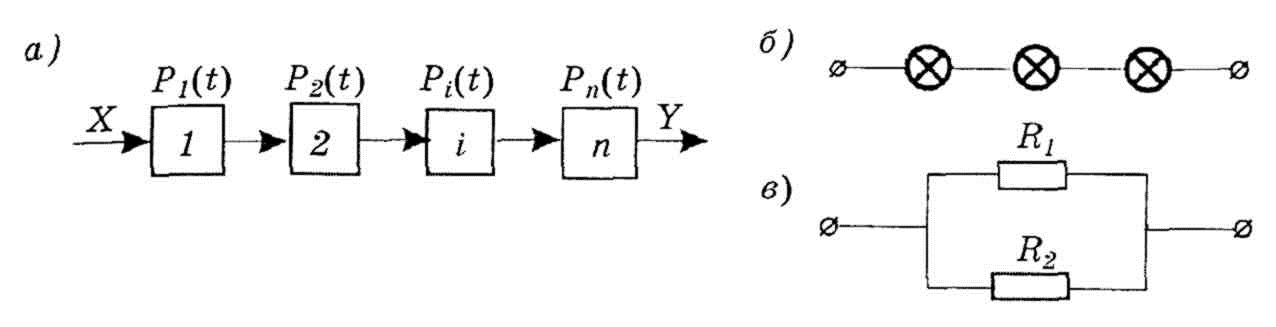
\includegraphics[width=1\textwidth]{13posled.png}
	\label{pic:13posled}
\end{figure}

При последовательном соединении $ n $ элементов (рис.~\ref{pic:13posled}~а) отказ системы наступает при отказе хотя бы одного из них, поэтому вероятность безотказной работы системы в течение времени $ t $ определяется (согласно правилу умножения вероятностей независимых событий) произведением вероятностей безотказной работы $ n $ ее элементов:
\[ P_\Sigma (t) = \prod\limits_{i=1}^{n}P_i(t). \]

Интенсивность отказов системы вычисляется по формуле:
\[ \lambda_\Sigma (t) = \sum\limits_{i=1}^{n}\lambda_i(t). \]

Среднее время безотказной работы:
\[ t_\text{ср} = \int\limits_{0}^{\infty} P_\Sigma (t)\,dt = \int\limits_{0}^{\infty} e^{-\lambda_\Sigma (t)\,t} dt = 
	\dfrac{1}{\lambda_\Sigma (t)} = \dfrac{1}{\sum\limits_{i}^{n} \lambda_i (t)} = \dfrac{1}{\sum\limits_{i=1}^{n}\dfrac{1}{t_{\text{ср}\,i}}}. \]

Для однотипных элементов, имеющих одинаковую вероятность безотказной работы всех элементов, например, при последовательном включении $ n $ лампочек елочной гирлянды (рис.~\ref{pic:13posled}~б) соответственно имеем:
\[ P_\Sigma(t) = P^n(t); \, \lambda_\Sigma = n\lambda; \, t_{\Sigma\,\text{ср}} = \dfrac{t_\text{ср}}{n}, \]
т.е. вероятность безотказной работы системы уменьшается с увеличением числа последовательно соединенных элементов, интенсивность отказов $ \lambda_\Sigma $ в $ n $ раз больше интенсивности отказов $ \lambda $ одного элемента, а среднее время безотказной работы в $ n $ раз меньше среднего времени безотказной работы одного элемента.

Следовательно, при проектировании прибора необходимо стремиться к возможно меньшему числу последовательно соединенных элементов и повышению надежности элементов, имеющих наиболее низкую вероятность безотказной работы (например, их резервированием).

Как уже было сказано, последовательность включения элементов в смысле надежности не эквивалентна последовательности их включения в функциональном смысле (для передачи информации, энергии). Например, система, изображенная на рис.~\ref{pic:13posled}~в с параллельно включенными резисторами $ R_1 $ и $ R_2 $ , выходит из строя при коротком замыкании одного из них.

Отказ системы при параллельном соединении элементов (рис.~\ref{pic:13par}~а) не возникает при отказе любого элемента и происходит только тогда, когда откажут все элементы.

\begin{figure}[h!]
	\caption{ Параллельное (в смысле надежности) соединение элементов прибора }
	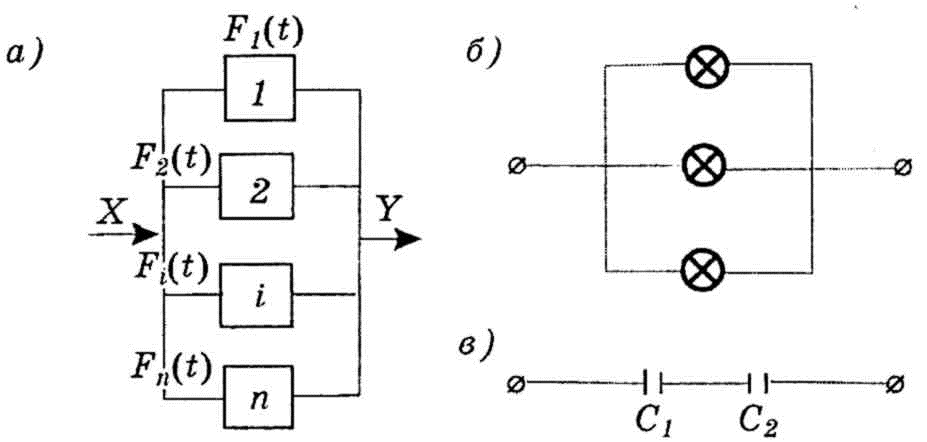
\includegraphics[width=0.7\textwidth]{13par.png}
	\label{pic:13par}
\end{figure}

Вероятность $ F_\Sigma (t) $ отказа системы в течение времени $ t $ в этом случае будет определена по формуле:
\[ F_\Sigma (t) = \prod\limits_{i=1}^{n}F_i (t), \]
где $ F_i(t) $ -- вероятность отказа i-ro элемента.

Следовательно, вероятность безотказной работы системы с параллельным соединением элементов:
\[ P_\Sigma (t) = 1 - F_\Sigma (t) = 1 - \prod\limits_{i=1}^{n} F_i (t). \]

При равнонадежных элементах, например, для елочной гирлянды с параллельным включением лампочек~(рис.~\ref{pic:13par}~б) имеем:
\[ F_\Sigma (t) = F_t^n; \, P_\Sigma(t) = 1 - F^n_t = 1 - [1-P(t)]^n. \]

Таким образом, резервирование является эффективным средством повышения надежности системы и особенно для этапа приработки прибора (вблизи $ t=0 $), где функция распределения случайного времени до первого отказа элементов обычно подчиняется экспоненциальному закону, поэтому:
\[ P_\Sigma (t) = 1 - (1 - e^{-\lambda\,t})^n. \]

Еще раз заметим, что параллельность соединения элементов в смысле надежности не всегда означает параллельность их соединения в функциональной структуре. Например, последовательное структурное соединение конденсаторов (рис.~\ref{pic:13par}~в) является параллельным в смысле надежности при коротком замыкании одного из них, когда их общая емкость не имеет значения (помехоподавляющий фильтр).

Примерами резервирования малонадежных элементов и систем являются следующие: дублирование источника освещения в медицинских операционных микроскопах; дублирование телевизионных камер в студиях, космических аппаратах.
\item Значительное количество отказов при эксплуатации приборов обусловлено ошибками операторов, вызванных ограниченными психофизиологическими возможностями человека, утомленностью, отступлением от привычных, стереотипных движений и расположений индикаторов, поэтому при проектировании приборов необходимо обеспечивать эргономические показатели их качества. Эти показатели характеризуют степень приспособленности прибора к взаимодействию с человеком с позиции удобства работы, гигиены, безопасности труда.
\end{enumerate}

%\section{Технологические мероприятия для повышения \\надежности}
При производстве приборов необходимо обеспечивать правильный выбор технологии производства, производить контроль и испытания качества материалов и продукции, соблюдать технологические режимы. Повысить надежность приборов можно за счет проведения следующих мероприятий.
\begin{enumerate}
\item  Применение рациональных видов и режимов обработки поверхностей деталей при технологической подготовке производства, позволяющих уменьшить шероховатость поверхностей, создать регулярный микрорельеф, повысить микротвердость (упрочнить) поверхностного слоя, что увеличивает износоустойчивость деталей, усталостную прочность, повышает коррозийную стойкость, уменьшает вероятность заедания и схватывания. К таким видам технологической обработки относятся, например, алмазное выглаживание и вибронакатывание поверхностей.
\item Контроль качества (т.е. физико-механических свойств) материалов и параметров комплектующих изделий. Необходимость проведения этого мероприятия вызвана тем, что поставляемые материалы и комплектующие могут отличаться по своим характеристикам и параметрам от запроектированных (например, погрешность датчиков может превосходить допустимое значение, класс точности подшипников более низкий, чем требуется, прочность материала может отличаться от требуемой).
\item Обеспечение культуры производства: чистоты оборудования и рабочего места, необходимых санитарных норм работы, защиты от вибраций, температурных и магнитных полей. Необходимость этого обусловлена тем, что данные факторы производства оказывают существенное (а иногда и доминирующее) влияние на качество продукции. Например, производство точных угловых растров (с погрешностью между штрихами не более 2-3 ) требует не только использования прецизионной делительной машины, но и установку ее на индивидуальном фундаменте, защиту от вибраций, стабилизацию давления и температуры до сотых долей градуса.
\item Строгое соблюдение технологического процесса, условий и режимов изготовления деталей и их сборки. Это требование обусловлено тем, что нарушение технологических процессов и условий может существенно снизить надежность изделий. Например, расклейки блоков линз или склеек их с оправами происходят обычно из-за того, что детали перед склейкой не были обезжирены или был использован клей с истекшим сроком применения.
\item Контроль по операциям при выпуске готовой продукции. Контроль деталей, узлов, компонентов приборов позволяет своевременно выявлять и исключать брак и тем самым повышать надежность прибора в целом. Например, в измерительном устройстве дальномера обязательной индивидуальной проверки и паспортизации требует местная погрешность шага микрометрического винта, так как в дальнейшем эта погрешность не компенсируется и может привести к отбраковке всего устройства или снижению точностной надежности дальномера.
\item Проведение разнообразных испытаний приборов (механических, климатических, термобарических, электрических, оптических) --- лабораторных, стендовых, полигонных, а также приемосдаточных, периодических и проверочных, которые позволяют выявить проектно-кон-структорские ошибки, дефекты изготовления и соответствие прибора требованиям ТУ, в том числе и показателям надежности.

Приемосдаточные испытания проводят в целях проверки каждого экземпляра прибора на соответствие ТУ, эталону и конструкторской документации.
Периодические испытания производят для проверки соответствия произвольно выбранных приборов (прошедших приемосдаточные испытания) требованиям технических условий в течение установленного времени, обычно не реже одного раза в год.

Типовые испытания проводят в целях оценки эффективности изменения принципиальной схемы, конструкции, технологии изготовления, используемых материалов и комплектующих, а также по рекламациям на приборы.
\end{enumerate}

\section[Эксплуатационные мероприятия для повышения надежности]{Эксплуатационные мероприятия для повышения \\надежности}
Для увеличения надежности приборов во время их эксплуатации необходимо учитывать следующие факторы, влияющие на надежность приборов, и обеспечивать соответствующие условия эксплуатации:
\begin{enumerate}
\item Так как эксплуатация прибора в непредусмотренных условиях и режимах является одним из основных источников отказов, не следует располагать приборы вблизи источников радиации, вибраций, силовых установок, воздействующих на прибор посредством механических и акустических полей. Режимы эксплуатации (временной, скоростной, силовой), условия и сроки обслуживания, поверки должны соответствовать инструкции.
\item В связи с тем, что интенсивность отказов наиболее высока в начальный период эксплуатации, целесообразно после хранения и транспортировки прибора, а также при его приобретении провести его тестирование и проверку на всех режимах работы (предпродажная подготовка).
\item Целесообразно подключать приборы к сети электрического питания через устройство стабилизации напряжения, а также обеспечивать их заземление.
\item Работать с приборами, осуществлять их своевременное обслуживание должен квалифицированный и ответственный персонал, подготовленный к работе с конкретными приборами. Усовершенствование и повышение квалификации персонала, его переподготовка, по возможности, должна осуществляться на фирме-производителе приборов или под ее руководством.
\item Необходимо создание специализированных служб по плановым проверкам, обслуживанию и ремонту приборов, осуществлению консультативной помощи персоналу.
\end{enumerate}